\noindent\textbf{\underline{\smash{Linear stability analysis}}}\\\vspace{0.2 cm}
Let $x^\ast$ be a fixed point and let $\eta(t)=x(t)-x^\ast$ be a small pertubation away from $x^\ast$. We are now interested whether the pertubation grows or decays:
\begin{equation*}
	\dot{\eta}=\frac{d}{dt}\left(x-x^\ast\right)=\dot{x} \quad \Rightarrow\quad \dot{\eta}=\dot{x}=f(x)=f(x^\ast+\eta)
\end{equation*}
We now expand $f(x)$ at $x^\ast$:
\begin{align*}
	f(x^\ast+\eta)&=\underset{=0}{f(x^\ast)}+\eta\frac{df}{dx}(x^\ast)+\mathcal{O}(\eta^2)\\
	\leadsto \dot{x}&=\dot{\eta}=\eta\frac{df}{dx}(x^\ast)+\mathcal{O}(\eta^2)
\end{align*}
Now, if $\frac{df}{dx}(x^\ast)\neq 0$ we can neglect the $\mathcal{\eta^2}$ terms and get
\begin{equation*}
	\dot{\eta}\approx\eta\frac{df}{dx}(x^\ast)
\end{equation*}
This equation is linear in $\eta(t)$ and called \textbf{linearization} about $x^\ast$. The pertubation $\eta(t)$ grow exponentially if $\frac{df}{dx}(x^\ast)>0$ and decays if $\frac{df}{dx}(x^\ast)<0$. This information has already been obtained by the graphical analysis. The new feature ist that we obtain a time scale $\frac{1}{\left|\frac{df}{dx}(x^\ast)\right|}$ which governs the exponential growth or decay.
\underline{\smash{Remark}}: In cases where $\frac{df}{dx}f(x^\ast)=0$ nothing can be said in general and we have to determine the stability on a case-by-case basis.
\underline{\smash{Examples}}:\\\vspace{0.1 cm}
\begin{figure}[H]
	\begin{tikzpicture}
		\draw[->] (-3,0)--(3,0);
		\draw[->] (0,-3)--(0,3);
		\draw[domain=-1.5:1.5,step=0.001] plot(\x,{-\x^3});
		\draw[fill=black] (0,0)circle(1pt);
		\node[right] at (0,1){(0,0) is stable};
	\end{tikzpicture}
	\begin{tikzpicture}
		\draw[->] (-3,0)--(3,0);
		\draw[->] (0,-3)--(0,3);
		\draw[domain=-1.5:1.5,step=0.001] plot(\x,{\x^3});
		\draw[fill=white] (0,0)circle(1pt);
		\node[left] at (0,1){(0,0) is unstable};
	\end{tikzpicture}\\
	\begin{tikzpicture}
		\draw[fill=black] (0,0)circle(1pt);
		\draw[white,fill=white] (0,-0.1)--(0,0.1)--(0.1,0.1)--(0.1,-0.1)--cycle;
		\draw[->] (-3,0)--(3,0);
		\draw[->] (0,-3)--(0,3);
		\draw[domain=-1.5:1.5,step=0.001] plot(\x,{(\x)^2});
		\draw (0,0)circle(1pt);
		\node[right] at (0,-1){(0,0) is halfstable};
	\end{tikzpicture}
	\begin{tikzpicture}
		\draw[->] (-3,0)--(3,0);
		\draw[->] (0,-3)--(0,3);
		\draw[fill=black] (-2,0)circle(1pt)(-1,0)circle(1pt)(0,0)circle(1pt)(1,0)circle(1pt);
		\node[right] at (0,1){all stable};
	\end{tikzpicture}
\end{figure}
\noindent So far we did not consider the existence and uniqueness of the solutions. The importance of that issue is illustrated by the following example:\\
\underline{Example}: Consider $\dot{x}=\sqrt[3]{x}$ and use tie initial condition $x_0=0$. The obvious solution is $x(t)=0$. But there is also another solution. Separating variables we get
\begin{equation*}
	\int x^{-\frac{1}{3}}=\int dt \leadsto \frac{3}{2}x^\frac{2}{3}+c=t
\end{equation*}
The initial condition leads to $c=0 \quad \leadsto \quad x(t)=\left(\frac{2}{3}t\right)^\frac{3}{2}$ is also a solution!\\
In case of a non-unique solution our analysis obiously fails!\\
So, we have to ask, which conditions are neccessary to obtain a unique solution.\\
\textbf{\underline{\smash{Exsitence and uniqueness theorem}}}: Consider the initial value problem
\begin{equation*}
	\dot{x}=f(x);\quad x(0)=x_0
\end{equation*}
Suppose that $f(x)$ and $\frac{df}{dx}(x)$ are continuous on an open interval $R$ of the $x$-axis and suppose that $x_0$ is a point in $R$. Then the initial value problem has a solution $x(t)$ on some time interval $]-\tau,\tau[$ about $t=0$, and the solution is unique.\\
\underline{\smash{Remark}}: Please note that the theorem does \textbf{not} imply that the solution exists for all times.\\
\underline{\smash{Example}}: $\dot{x}=1+x^2; \quad x(0)=x_0$. The uniqueness theorem applies for all values $x_0$ since $f(x)$ and $\frac{df}{dx}(x)$ are continuous. But for $x_0=0$ we get:
\begin{equation*}
	\int \frac{1}{1+x^2}dx=\int dt \leadsto t=\arctan(x)+c
\end{equation*}
$\leadsto c=0$ \& $x(t)=tan(t)$. Obviously $x$ diverges for $t\to\frac{\pi}{2}$, i.e. in finite time!\\
\underline{\smash{Remark}}: FP dominate the dynamics of 1st order systems in one dimension. More specifically trajectories either approach a fixed point or diverge to $\pm\infty$. These are actually the only things that may happen to a vector field on a real line. In particular, trajectories cannot reverse direction (oscillate) since they had to cross a fixpoint. \textbf{Potentials} provide another possibility to characterize a dynamic system graphically. We introduce a potential via $f(x)=-\frac{dV}{dx}$, using this picture one should consider the particle damped, its inertia completely negligible. As in physics, the particle always moves downhill.
\begin{align*}
	\frac{dV}{dt}&=\frac{dV}{dx}\frac{dx}{dt}\qquad\&\qquad\frac{dx}{dt}=f(x)=-\frac{dV}{dx}\\
	\leadsto \frac{dV}{dt}&=-\left(\frac{dV}{dx}\right)^2 \leadsto V \text{ always decreases along trajectories}
\end{align*}
At an equilibrium point we have $\frac{dV}{dt}=0$. Local minima correspond to stable fixpoints, local maxima to unstable fixpoints.\\
\underline{\smash{Example}}: $\dot{x}=\underset{f(x)}{\underbrace{x-x^3}} \leadsto V(x)=-\frac{1}{2}x^2+\frac{1}{4}x^4+c$
\begin{figure}[H]
	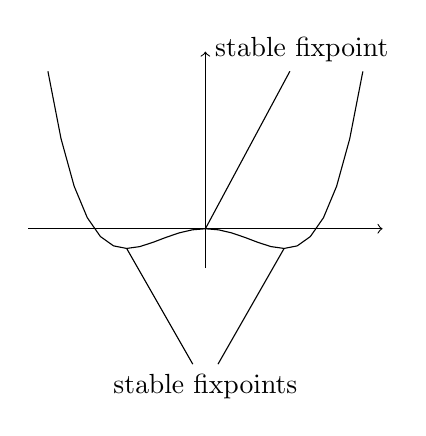
\begin{tikzpicture}
		\draw[->] (-2.25,0)--(2.25,0);
		\draw[->] (0,-0.5)--(0,2.25);
		\draw[domain=-2:2,step=0.001] plot(\x,{-0.5*(\x)^2+(\x)^4/4});
		\node[name=s] at (0,-2){stable fixpoints};
		\node[name=u,above right] at (0,2){stable fixpoint};
		\draw (-1,-0.25)--(s)(1,-0.25)--(s);
		\draw (0,0)--(u);
	\end{tikzpicture}
\end{figure}
\textbf{\underline{\smash{Bifurcations}}}: 1D flows are simle: Either they converge to a fixed point or head on to $\pm\infty$. The most interesting aspect of 1D flows is their parameter dependence.\\
Qualitative changes of the dynamics upon variation of the parameters are called \textbf{bifurcations}, and the corresponding parameter \textbf{values} are called \textbf{bifurcation points}.\\
\textbf{Saddle-Node-Bifurcation}
\begin{itemize}[label={$\cdot$}]
	\item Basic machanism by which fixpoints are created or destroyed\\
		Introductory example $\dot{x}=r+x^2$
		\begin{figure}[H]
			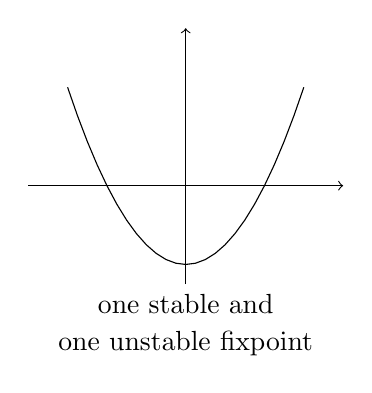
\begin{tikzpicture}
				\draw[->](-2,0)--(2,0);
				\draw[->](0,-1.25)--(0,2);
				\draw[domain=-1.5:1.5,step=0.001] plot(\x,{-1+(\x)^2});
				\node at (0,-1.5){one stable and};
				\node at (0,-2){one unstable fixpoint};
			\end{tikzpicture}
			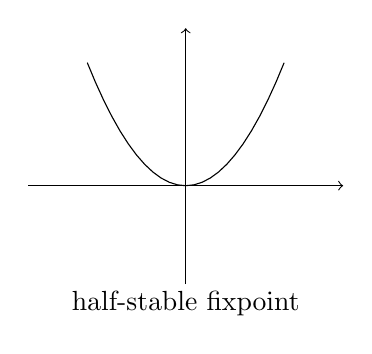
\begin{tikzpicture}
				\draw[->](-2,0)--(2,0);
				\draw[->](0,-1.25)--(0,2);
				\draw[domain=-1.25:1.25,step=0.001] plot(\x,{(\x)^2});
				\node at (0,-1.5){half-stable fixpoint};
			\end{tikzpicture}
			\begin{tikzpicture}
				\draw[->](-2,0)--(2,0);
				\draw[->](0,-1.25)--(0,2);
				\draw[domain=-1:1,step=0.001] plot(\x,{1+(\x)^2});
				\node at (0,-1.5){no fixpoint};
			\end{tikzpicture}
		\end{figure}
		The fixpoints are located on the curve $r=-x^2$
		\begin{figure}[H]
			\begin{multicols}{2}
				\begin{figure}[H]
					\centering
					\begin{tikzpicture}
						\draw [->] (-2,0)--(2,0);
						\draw[->] (0,-2)--(0,1);
						\draw[domain=-1.5:1.5,step=0.001] plot(\x,{-(\x)^2});
					\end{tikzpicture}
				\end{figure}\columnbreak
				Typically the axes are inverted since $r$ is the independent variable\\
				Bifurcation diagram:\\
				\begin{figure}[H]
					\begin{tikzpicture}
						\draw[->](-2,0)--(1,0);
						\draw[->](0,-2)--(0,2);
						\draw[domain=-2:0,step=0.001] plot(\x,{-sqrt(-\x)});
						\draw[domain=-2:0,step=0.001,dashed] plot(\x,{sqrt(-\x)});
						\node[right] at (0,1){saddle-node bifurcation};
					\end{tikzpicture}
				\end{figure}
			\end{multicols}
		\end{figure}
\end{itemize}
\underline{\smash{Example}}: We consider the 1st order system $\dot{x}=r-x-e^{-x}=f(x)$\\
For this choice of $f(x)$ the fixpoints are difficult to obtain analytically. But we notice the following: fixpoints are located where the two curces $e^{-x}$ and $r-x$ intersect upon variation of $r$ we get:
\begin{figure}[H]
	\begin{tikzpicture}
		\draw[->] (-3,0)--(3,0);
		\draw[->] (0,-1)--(0,3);
		\draw[domain=-1.15:3,step=0.001] plot(\x,{exp(-\x)});
		\draw[domain=-2:2,step=0.001] plot(\x,{1-\x});
		\draw[domain=-1:3,step=0.001,dashed] plot(\x,{1.8-\x});
		\draw[domain=-3:1,step=0.001,dashed] plot(\x,{0.2-\x});
	\end{tikzpicture}
\end{figure}
